\part{User Manual}\label{part2}
It is assumed that the reader has studied the MCLab Handbook before using CSAD, and has knowledge about Lab equipment, procedures and Safety precautions. In addition, the following is important to keep in mind when using CSAD:
\begin{description}
	\item [{Water~damage:}] CSAD is watertight when the hatches on the top are closed properly.  
	\item [{Propeller~dry~running:}] The thruster gears are lubricated with water, and thus the propellers always has to be in the water when running. Hence, always keep the vessel in the basin when the power is connected. 
	\item [{Loss~of~laptop~control:}] Wireless network instability may result in loss of connection between the laptop user interface and the cRIO. In this event, fall back to manual thruster control, by pushing 
\includegraphics[scale=0.4]{fig/sixaxis_triangle} on the Sixaxis, or alternatively press 
\includegraphics[scale=0.4]{fig/sixaxis_circle} to stop the vessel. 
	\item [{Total~loss~of~control:}] Pull CSAD with a boat hook, and keep the vessel in water while disconnecting batteries.
	\item [{Launching}] CSAD is a large model, and care must be taken when launching the vessel to the basin. Always be two persons, and make sure the vessel does not hit the basin wall when launching or removing it from the basin. When launching, remove all weights(batteries and ballast). Still, the vessel is heavy, and the lifting up and down to the basin might be harder than expected. 
\end{description}
\chapter{Launching}
\section{Update customized simulink code}
In the MC-Lab Handbook, a description on how to compile and upload the customized Simulink code is given. Here is only the specific application for CSAD given. All necessary files to control CSAD is found on GitHub: \url{https://github.com/NTNU-MCS/CS_Drillship_cRIO}. Download the folder with all files, and follow the instructions in MC-Lab Handbook for implementing your control system in the VeriStand project. 

After successfully implementing the customized simulink code in the VeriStand project, continue to the next Section. 

\section{Vessel and lab preparations}
Follow these vessel-specific instructions when preparing for experiments with CSAD: 
\begin{enumerate}
	\item Make sure all batteries and weights are removed from the vessel when lifting it. Launch the vessel in the basin. 
	\item Place all 6 batteries(12V 12Ah, marked CSAD) in the vessel, at their dedicated places. 3 in front of the moonpool, 3 behind it. Connect the batteries, positive/7red first then negative/black. 
	\item Place the ballast weights. 20 kg in the aft, and 27.5 in the front. Manually adjust their position, such that the vessel does not have any heel (slagside). Check with the design draft indicated on the outside of the hull. 
	\item Turn on the power switch. This is located on the backside of the plastic box containing the cRIO. It might be a bit hard to find at first, use your left hand and search with your fingers around the centerline. 
	\item Verify that the WiFi-bridge connects, the blue light is continuous. 
	\item Once the bluetooth dongle connected to the RPi starts blinking(frequency of 1 Hz), press the PS-button on the Sixaxis. On the controller, indicator 1 lights continuously red when successfully connected. 
	\item Place the vessel inside the region of sight for Qualisys (check on the Qualisys computer that all 4 reflectors are visible for all cameras). Align the vessel with 0\degree heading in the basin frame, i.e. with the bow pointing towards the command center. 
	\item On the Qualisys computer, aqcuire the body. This process is described in MC-Lab Handbook, with information on debugging. In the body frame, the highest marker has position $(x,y,z)=(960,-190,-575)[mm]$. 
	\item Go to 3D Visualization in QTM, and verify that the body is correct. The body x-axis should be parallel to the lines between the markers on starboard and port side.
\end{enumerate}
CSAD and the lab is now set up for experiments. 
\section{Upload VeriStand project to the vessel}
With the hardware prepared, follow these instructions to upload the VeriStand project to the cRIO onboard CSAD. 
\begin{enumerate}
	\item Make sure the computer is connected to the MC-Lab network(either by Ethernet cable or the WiFi). 
	\item Check the communication between the laptop and CSAD. Open Command Prompt(\textit{cmd.exe}), write the following: \texttt{ping 192.168.0.55}. The response time varies, but it is crucial that the command returns 0\% loss. 
	\item Open the VeriStand project (\textit{CSAD.nivsproj}). If the project has been updated as described in the MC-Lab Handbook, press the deploy button (see Figure \ref{fig:project_explorer}). The code is then uploading to the cRIO onboard the vessel. If the deployment is not successful, verify that the sixaxis controller is connected to the RPi and that the body is tracked in Qualisys. Try deploying again. If it still does not work, try restarting the vessel (either resetting the power switch in the vessel, or restart the cRIO in NI MAX). Also check that the Qualisys computer is connected to the same network(\texttt{ping 192.168.0.10}). 
	\item When successfully deployed project, open the Workspace (\textit{CSAD.nivsscreen}) as shown in Figure \ref{fig:project_explorer}. The code is now running on the cRIO, continue to the next Chapter for instruction on operating the vessel. 
\end{enumerate}
\begin{figure}[h!]
	\centering
	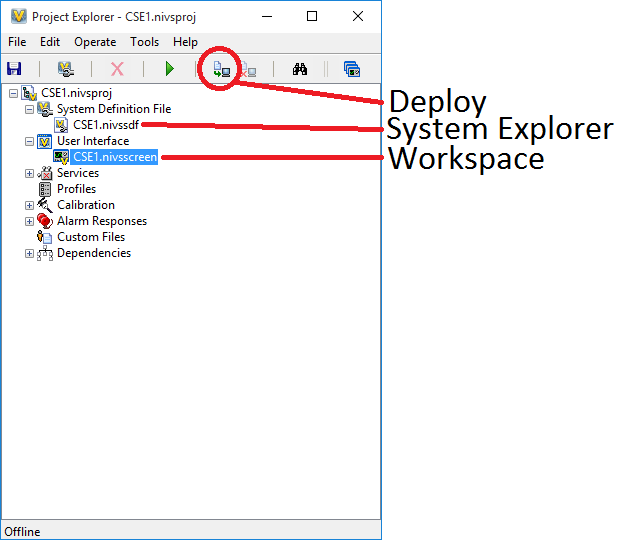
\includegraphics[width=0.8\textwidth]{fig/project_explorer.png}
	\caption{User interface in VeriStand Project Explorer}
	\label{fig:project_explorer}
\end{figure}

\chapter{Operating}
After successful deployment of the VeriStand project, you control the vessel with the sixaxis-controller and/or the laptop. The sixaxis controller works as the main controller, and thus always have the sixaxis controller at hand in case of error in your control system. Use the sixaxis controller to switch between the different operation modes: 
\begin{itemize}
	\item 
\includegraphics[scale=0.4]{fig/sixaxis_triangle} - ctrl\_sixaxis2thruster
	\item 
\includegraphics[scale=0.4]{fig/sixaxis_square} - ctrl\_custom
	\item 
\includegraphics[scale=0.4]{fig/sixaxis_cross} - ctrl\_DP
	\item 
\includegraphics[scale=0.4]{fig/sixaxis_circle} - STOP
\end{itemize}
\section{Workspace}
On the laptop, use the Workspace to monitor and control the different parameters in the Simulation models. There are 1 screen for each operation mode. You should not alter the screen for ctrl\_sixaxis2thruster or ctrl\_DP, while the ctrl\_custom can be modified as desired. How to use and modify the Workspace is described in the MC-Lab Handbook.

Data logging can be done in two ways, as described in MC-Lab Handbook.  
\chapter{Demolition}
When the experiments are finished, follow the procedure given here to shut down. 
\begin{enumerate}
	\item Switch to \textit{ctrl\_sixaxis2thruster}, and navigate CSAD near the basin wall
	\item In the Project Explorer window, press to undeploy the code
	\item Turn of the power switch, and disconnect the batteries
	\item Remove the ballast weights
	\item Remove the batteries from the vessel
	\item Lift CSAD from the basin, and put it in its rack in the storage
	\item Leave the sixaxis controller in the vessel
	\item On the Qualisys computer, quit Qualisys Track Manager
	\item If you recorded any videos with the Camera System, export these videos to a memory stick, quit the software and turn of the TV-monitor
	\item Do a general clean up, bring all your personal belongings with you when you leave
\end{enumerate}
NOTE on charging the batteries: When charging the batteries in CSAD, the WiFi bridge must be disconnected. Unplug the power wire from the WiFi bridge(connected on the side of the Ethernet cable). All batteries must be placed in the vessel when charing, and connected, but with the power switch turned off. Connect the charger to the charging wire located in the aft hatch. The charger is located in the shelf in the storage, marked CSAD. Set the charging mode to the motorcycle symbol. 